\documentclass[aspectratio=169]{beamer}

%%% Работа с русским языком
\usepackage{cmap}					% поиск в PDF
\usepackage{mathtext} 				% русские буквы в формулах
\usepackage[T2A]{fontenc}			% кодировка
\usepackage[utf8]{inputenc}			% кодировка исходного текста
\usepackage[english,russian]{babel}	% локализация и переносы
\usepackage{indentfirst}
\frenchspacing

%%% Дополнительная работа с математикой
\usepackage{amsmath,amsfonts,amssymb,amsthm,mathtools}  % AMS

%%% Текст в колонки
\usepackage{multicol}

%%% Системы уравнений
\usepackage{cases}

%%% Таблицы
\usepackage{array}

%%% Картинки
\usepackage{graphicx}
\usepackage{float}

%%% Список литературы
\usepackage[
	sorting = none,
	language = autobib,
	autolang = other
]{biblatex}
\renewbibmacro{in:}{\ifentrytype{article}
    {}
    {\bibstring{in}\printunit{\intitlepunct}}
}
\addbibresource{references.bib}

%%% Гиперссылки
\usepackage{hyperref}

%%% Прямой знак интеграла
\usepackage[integrals]{wasysym}

%%% Перенос знаков в формулах (по Львовскому)
\newcommand*{\hm}[1]{#1\nobreak\discretionary{}
{\hbox{$\mathsurround=0pt #1$}}{}}


%%% Свои команды

\newcommand{\vect}[1]{\textbf{#1}}
\newcommand{\vx}{{\vect{x}}}
\newcommand{\vn}{{\vect{n}}}

\newcommand{\half}{\cfrac{1}{2}}

\newcommand{\partt}[1]{\cfrac{\partial #1}{\partial t}}
\newcommand{\partvn}[1]{\cfrac{\partial #1}{\partial \vn}}

\newcommand{\partflt}[1]{\partial #1 / \partial t}
\newcommand{\partflvn}[1]{\partial #1 / \partial \vn}

\newcommand{\gradsq}[1]{(\nabla #1, \nabla #1)}

\newcommand{\Natural}{{\mathbb{N}}}
\newcommand{\Real}{{\mathbb{R}}}
\newcommand{\bigO}{{\mathcal{O}}}
\newcommand{\clOmega}{{\overline{\Omega}}}

\newcommand{\taumin}{{\tau_{\min}}}
\newcommand{\taumax}{{\tau_{\max}}}

\newcommand{\parind}{\hspace{7.5mm}}
\newcommand{\tabularitem}[2]{%
\begin{itemize}
	\begin{minipage}[c][#1]{\hsize} \item #2 \end{minipage}
\end{itemize}%
}

\newcommand{\nologo}{\setbeamertemplate{logo}{}}


%%% Свои операторы
\DeclareMathOperator{\Div}{{div}}
\DeclareMathOperator{\Const}{{const}}
\DeclareMathOperator{\Tol}{{tol}}

%%% Тема оформления
\usetheme{Madrid}


%%% Титульный лист
\title[Адаптация шага по времени]{Адаптация расчетного шага по времени \\ в трехмерной постановке задачи развития канала \\ электрического пробоя}
\author[]{
	Пономарев А. С.\textsuperscript{1,2}, Зипунова Е. В.\textsuperscript{2}, Савенков Е. Б.\textsuperscript{2}
}
\institute[МФТИ, ИПМ]{
	\textsuperscript{1}МФТИ (НИУ) \\
	\textsuperscript{2}ИПМ им. М. В. Келдыша РАН
}
\date[68-я Конференция МФТИ]{
	68-я Всероссийская научная конференция МФТИ \\[1mm]
	30.03.2026
}
\logo{
\includegraphics[height=0.8cm]{../figures/labels.jpg}}


\begin{document}

\AtBeginSection[]{
	\begin{frame}{Содержание}
	\Large
	\tableofcontents[currentsection]
	\end{frame}
}

\begin{frame}
\titlepage
\end{frame}


%!TEX root = ../main.tex

\section{Постановка задачи}

\begin{frame}{Математическая модель}
\begin{block}{Модель типа диффузной границы}
	Вещество находится в разных фазах. Состояние вещества описывается гладкой функцией $\phi(\vx, t)$ -- фазовым полем.
\end{block}
\begin{itemize}
	\item $\phi = 1$ -- неповрежденная среда
	\item $\phi = 0$ -- полностью разрушенная среда
	\item Зона $\phi \in (0, 1)$ -- диффузная граница
	\item На разрушение среды тратится энергия
\end{itemize}
\begin{figure}
	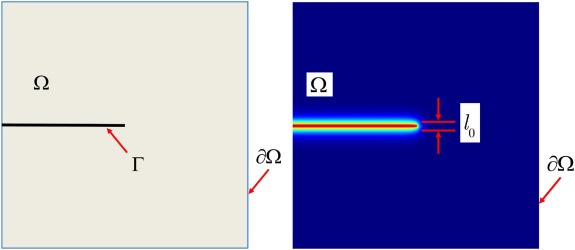
\includegraphics[width=0.5\textwidth]{figures/diffuse_edge.jpg}
\end{figure}
\end{frame}


\begin{frame}{Математическая модель}
%\vspace{-0.3cm}
\begin{block}{Уравнения динамики системы}
	\begin{gather*}
		\Div(\epsilon[\phi] \nabla \Phi) = -\rho_E \\
		\partt{\rho_E} = \Div(\sigma[\phi] \nabla \Phi) \\
		\cfrac{1}{m} \partt{\phi} = -F'( \phi; \| \nabla \Phi \|) + \cfrac{\Gamma}{2} \Delta \phi + \beta \Gamma l^2 \Div \left( \| \nabla \phi \|_2^2 \nabla \phi \right)
	\end{gather*}
\end{block}
\begin{itemize}
	\item Плотность свободной энергии Гельмгольца
	\vspace{-0.2cm}
	\[
		\pi = F( \phi; \| \nabla \Phi \|) + \cfrac{\Gamma}{4} \| \nabla \phi \|_2^2 + \cfrac{\beta}{4} \Gamma l^2 \| \nabla \phi \|_2^4
	\]
	\item $m$, $\Gamma$, $l$ -- параметры модели, константы
\end{itemize}
\end{frame}


\begin{frame}{Математическая модель}
\begin{gather*}
	F(\phi; \| \nabla \Phi \|) = -\half \epsilon[\phi] \cdot \| \nabla \Phi \|_2^2 + \Gamma \cfrac{1 - f(\phi)}{l^2} \\
	\begin{alignedat}{3}
		\epsilon[\phi] &= \epsilon(\vx, t) &&= \cfrac{\epsilon_0(\vx)}{f(\phi(\vx, t)) + \delta} \\
		\sigma[\phi] &= \sigma(\vx, t) &&= \cfrac{\sigma_0(\vx)}{f(\phi(\vx, t)) + \delta}
	\end{alignedat} \\[2mm]
	f(\phi) = 4 \phi^3 - 3 \phi^4
\end{gather*}
\vspace{-3mm}
\begin{itemize}
	\item $\delta$ -- регуляризующий параметр
	\item $f(\phi)$ -- интерполирующая функция
\end{itemize}
\end{frame}


\begin{frame}{Разностная схема}
\vspace{-5mm}
\begin{enumerate}
	\item $\; \Div_h \left( \epsilon[\phi] \nabla_h \hat{\Phi} \right) = - \rho_E \quad \leadsto \quad \hat{\Phi}$
	\item $\left[ \partt{\phi} \right]_h = m \cdot \left( -F'( \phi; \| \nabla_h \hat{\Phi} \|) + \cfrac{\Gamma}{2} \Delta_h \phi + \beta \Gamma l^2 \Div_h \left( \| \nabla_h \phi \|_2^2 \nabla_h \phi \right) \right)$
	\item $\left[ \partt{\rho} \right]_h = \Div_h \left( \sigma[\phi] \nabla_h \hat{\Phi} \right)$
	\item $\hat{\phi} = \phi + \tau \cdot \left[ \partt{\phi} \right]_h; \qquad \hat{\rho}_E = \rho_E + \tau \cdot \left[ \partt{\rho} \right]_h$
\end{enumerate}
\end{frame}


\begin{frame}{Цель работы}
\vspace{-3mm}
\begin{center}
\begin{minipage}{0.95\textwidth}
\begin{block}{Цель работы}
	Исследовать применение адаптивного шага по времени при расчете задачи в полной, трехмерной постановке
\end{block}
\end{minipage}
\end{center}
\vspace{3mm}
\hspace{8mm} Требования к алгоритму адаптации:
\begin{itemize}
	\item Простота реализации
	\item Малый объем дополнительных вычислений
\end{itemize}
\end{frame}

%!TEX root = ../main.tex

\section{Метод адаптации}

\begin{frame}{Адаптация по фазовому полю}
\begin{block}{Формула расчета адаптивного шага}
	\[
		\tau^k = \max \left[ \taumin, \min \left( \taumax, \cfrac{\Tol}{\left\| [\partflt{\phi}]_h \right\|_C} \right) \right]
	\]
\end{block}
\vspace{3mm}
\parind Идея метода:
\[
	\| \hat{\phi} - \phi \|_C = \tau^k \cdot \left\| \left[ \partt{\phi} \right]_h \right\|_C = \cfrac{\Tol}{\left\| [\partflt{\phi}]_h \right\|_C} \cdot \left\| \left[ \partt{\phi} \right]_h \right\|_C \approx \Tol
\]
\parind Предложен в статье \cite{li_time_step}
\end{frame}

%!TEX root = ../main.tex

\section{Вычислительный эксперимент}


\begin{frame}{Граничные условия}
\centering
Кубический образец диэлектрика, зажатый между двумя проводящими пластинами. \\[5mm]
\begin{tabular}{m{0.5\textwidth} m{0.5\textwidth}}
	\parind Обкладки сверху и снизу: & \parind Боковая граница $\partial \Omega$: \\
	\tabularitem{12mm}{$\Phi|_{z = 0} = \Phi^+; \; \Phi|_{z = L} = \Phi^-$} &
	\tabularitem{12mm}{$\partvn{\Phi}\bigg|_{\partial \Omega} = 0$} \\
	\tabularitem{12mm}{$\cfrac{\partial \phi}{\partial z}\bigg|_{z = 0} = \cfrac{\partial \phi}{\partial z}\bigg|_{z = L} = 0$} &
	\tabularitem{12mm}{$\phi|_{\partial \Omega} = 1$}
\end{tabular}
\end{frame}


\begin{frame}{Расчет №1: <<иголка>>}
\vspace{-5mm}
\begin{figure}
	\subfloat[Начальное условие]{\frame{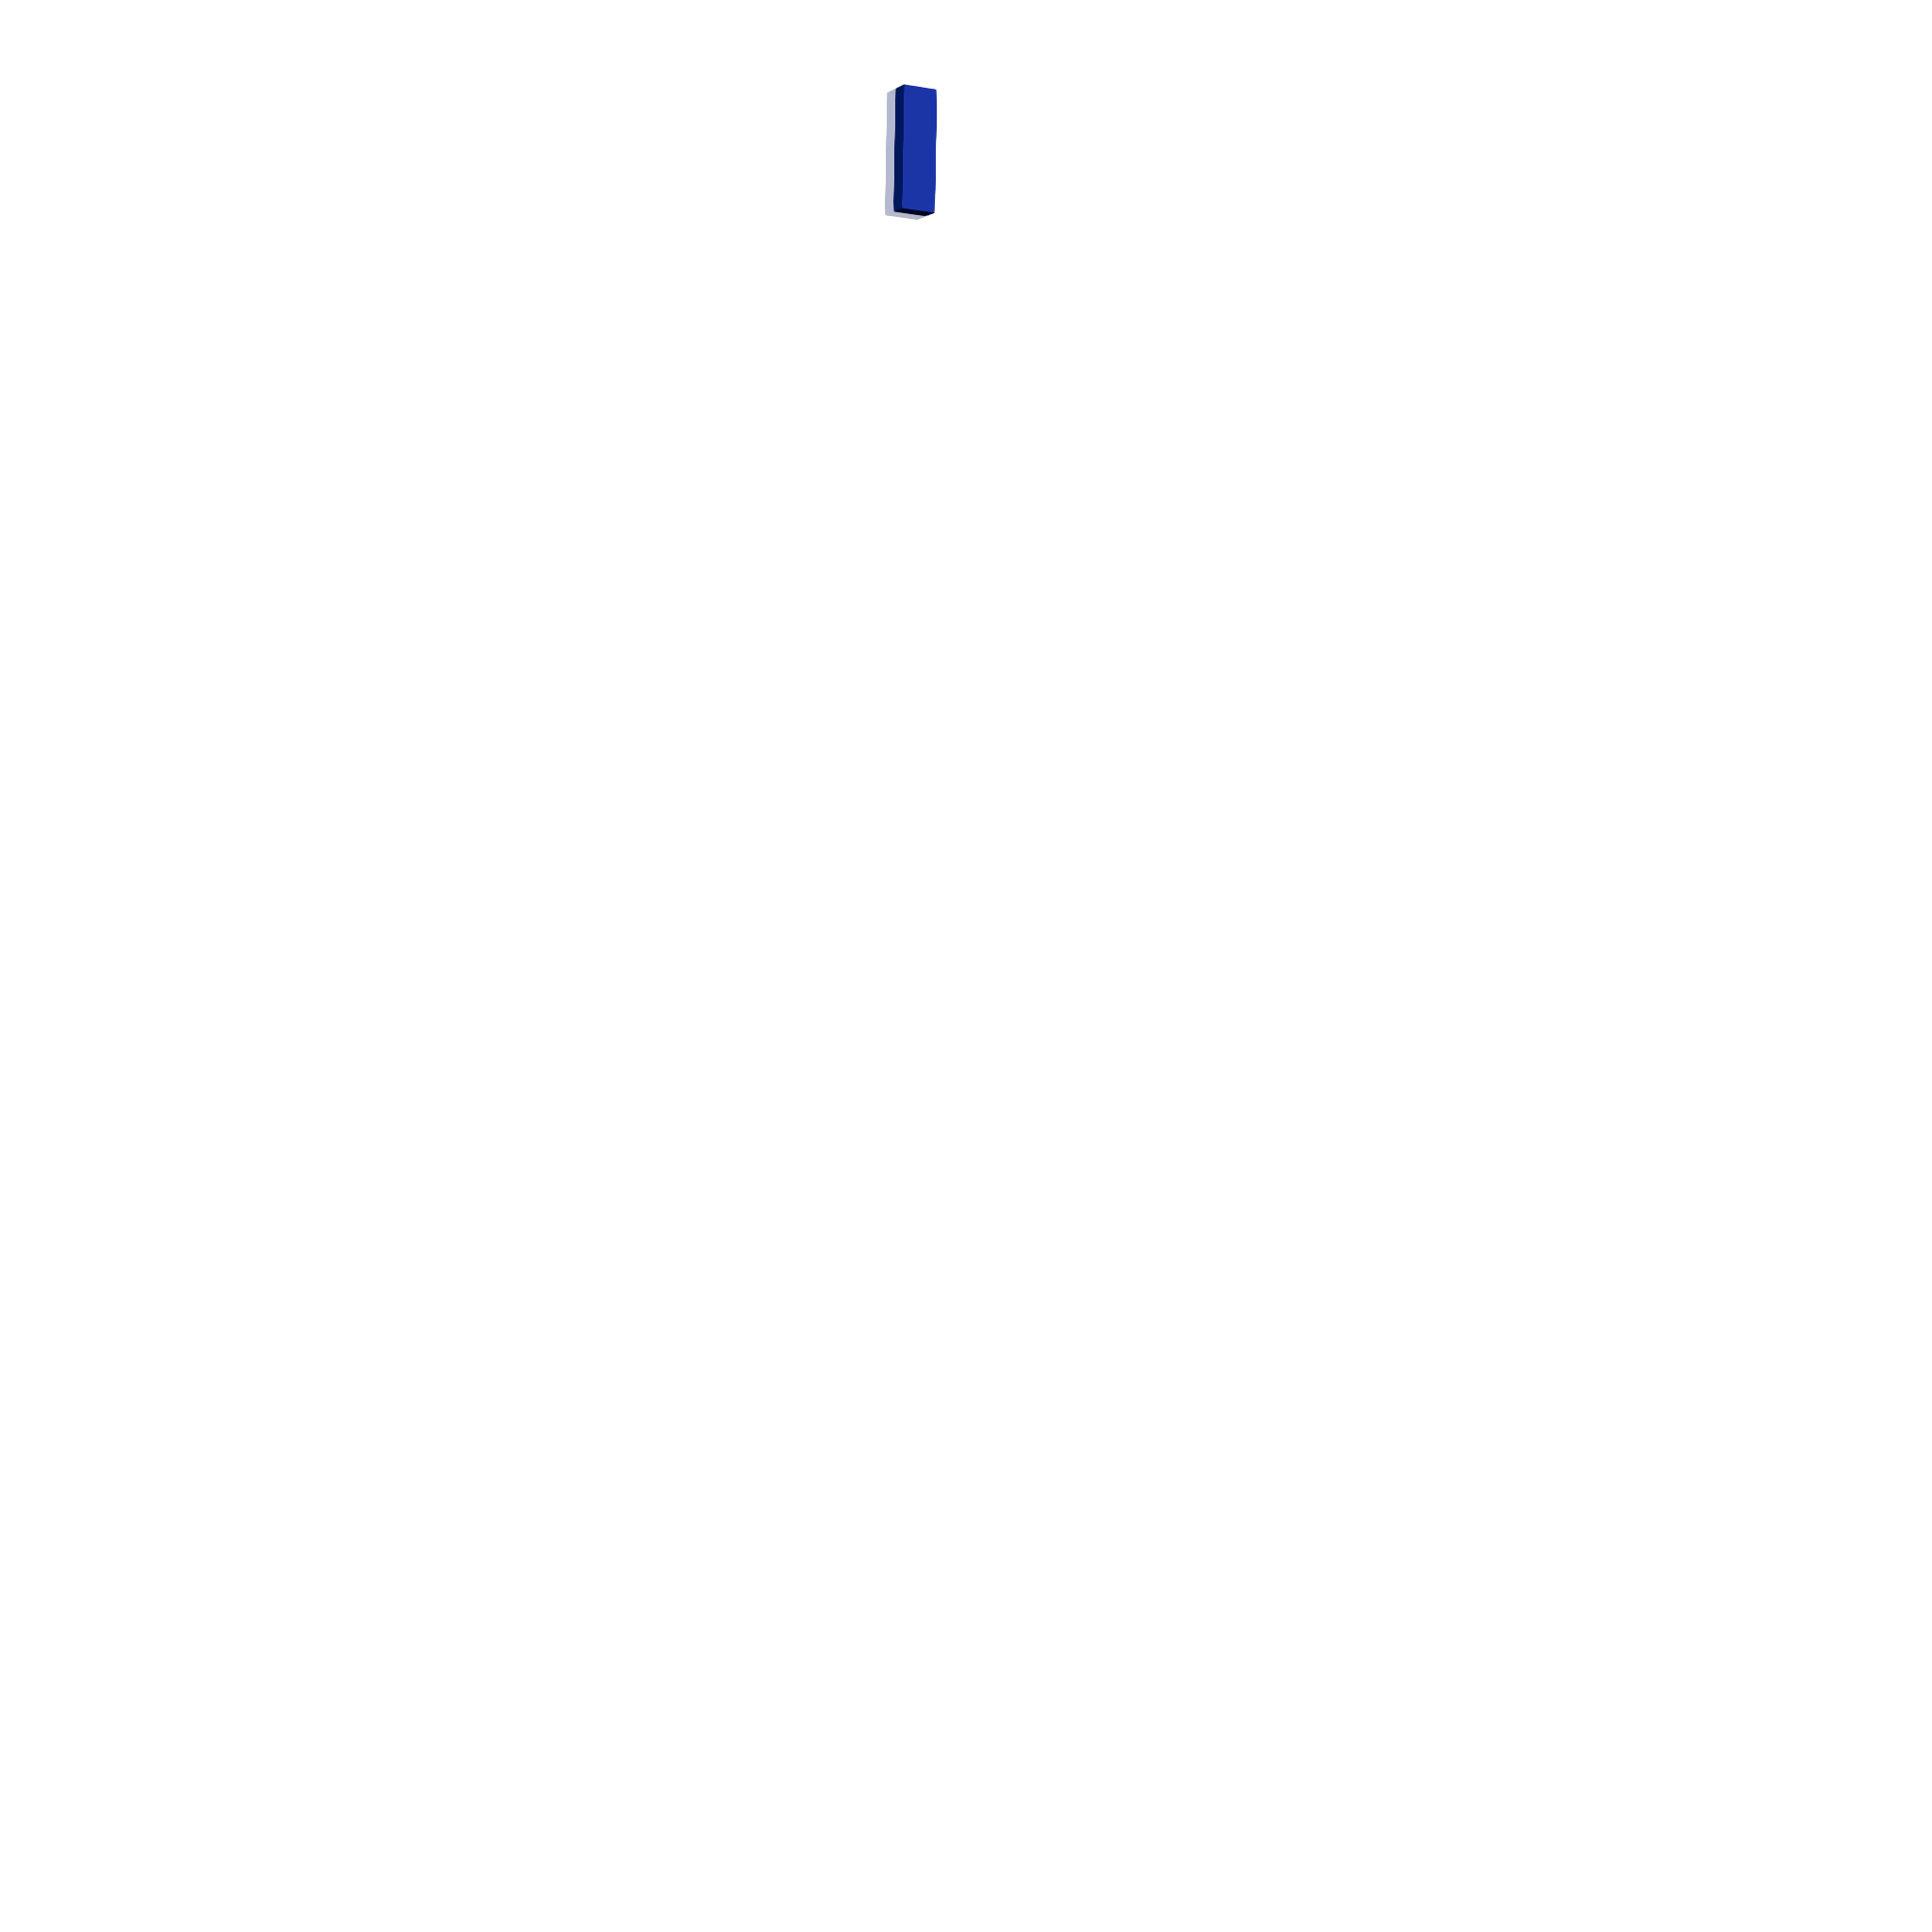
\includegraphics[width=0.333\textwidth]{figures/result_needle_0.png}}}
	\subfloat[Рост канала]{\frame{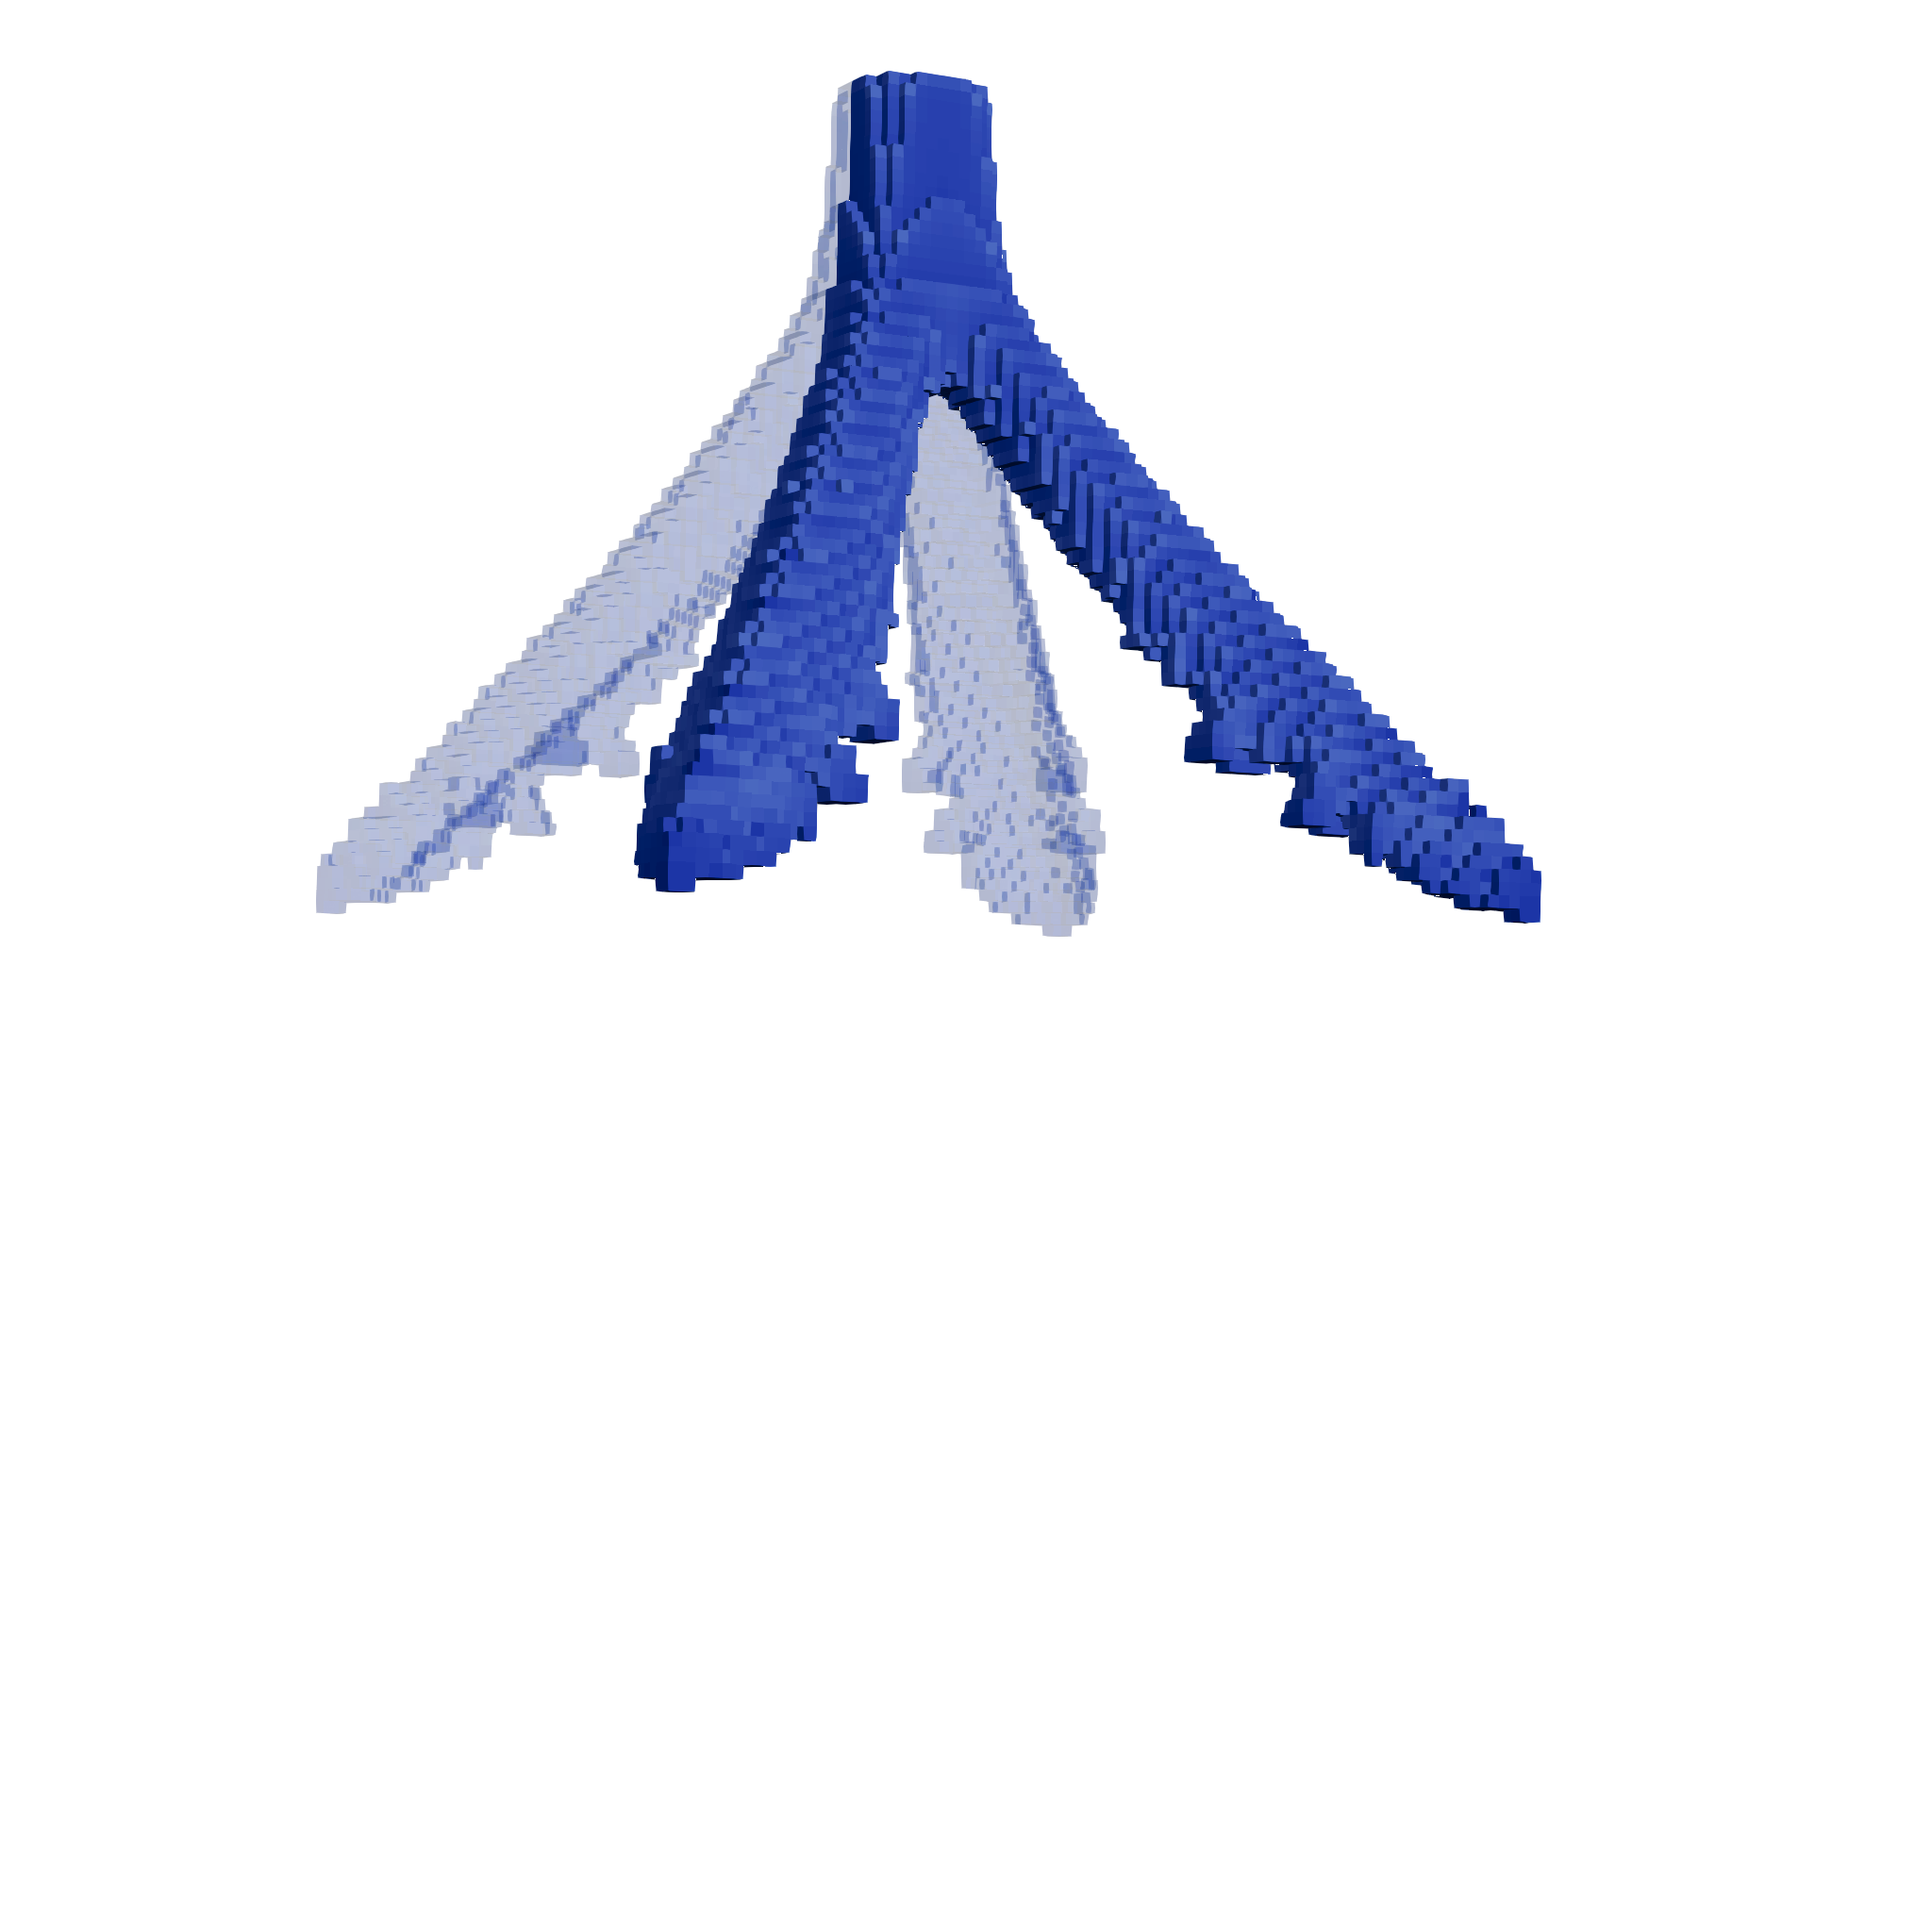
\includegraphics[width=0.333\textwidth]{figures/result_needle_1.png}}}
	\subfloat[Перед пробоем <<насквозь>>]{\frame{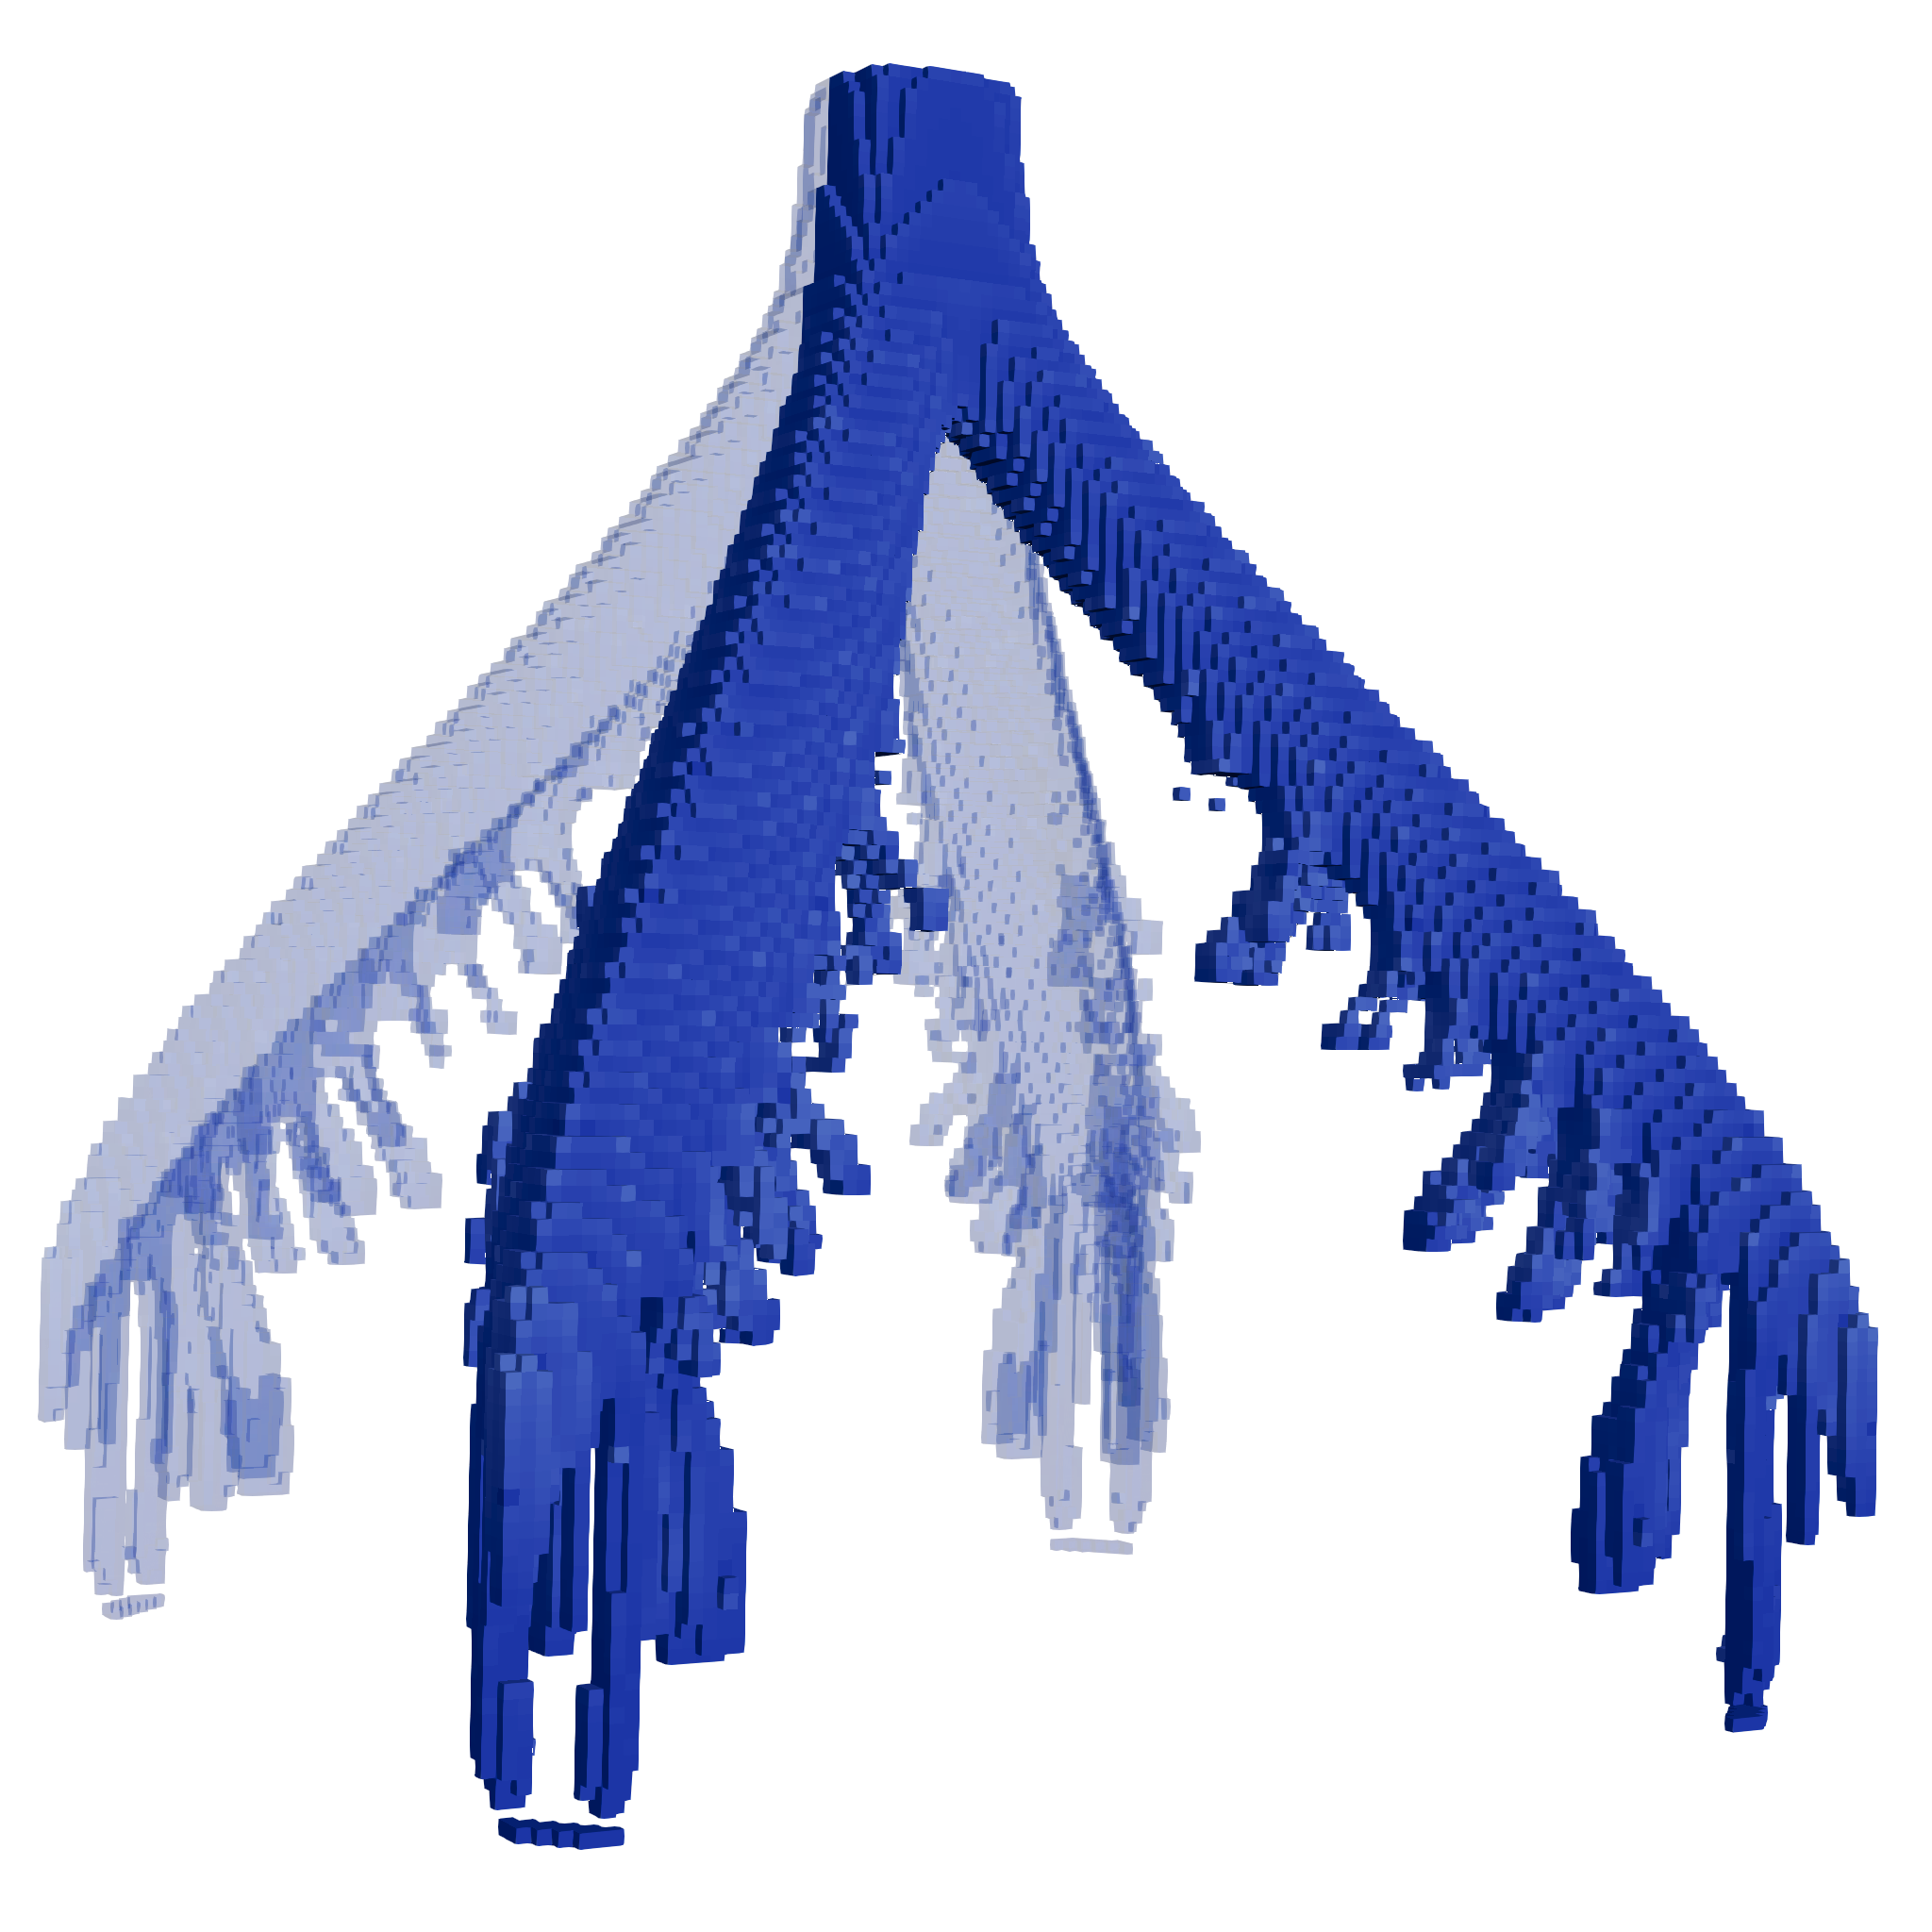
\includegraphics[width=0.333\textwidth]{figures/result_needle_2.png}}}
\end{figure}
\vspace{-7mm}
\begin{minipage}[l]{0.66\textwidth}
\begin{align*}
	N_h &= 129 & T &\approx 7 \cdot 10^{-7} & \taumin &= 10^{-12} \\
	N_t &= 51000 & \Tol &= 10^{-2} & \taumax &= 10^{-7}
\end{align*}
\end{minipage}
\end{frame}


\begin{frame}{Расчет №2: случайные возмущения}
\vspace{-5mm}
\begin{figure}
	\subfloat[Зародыши каналов]{\frame{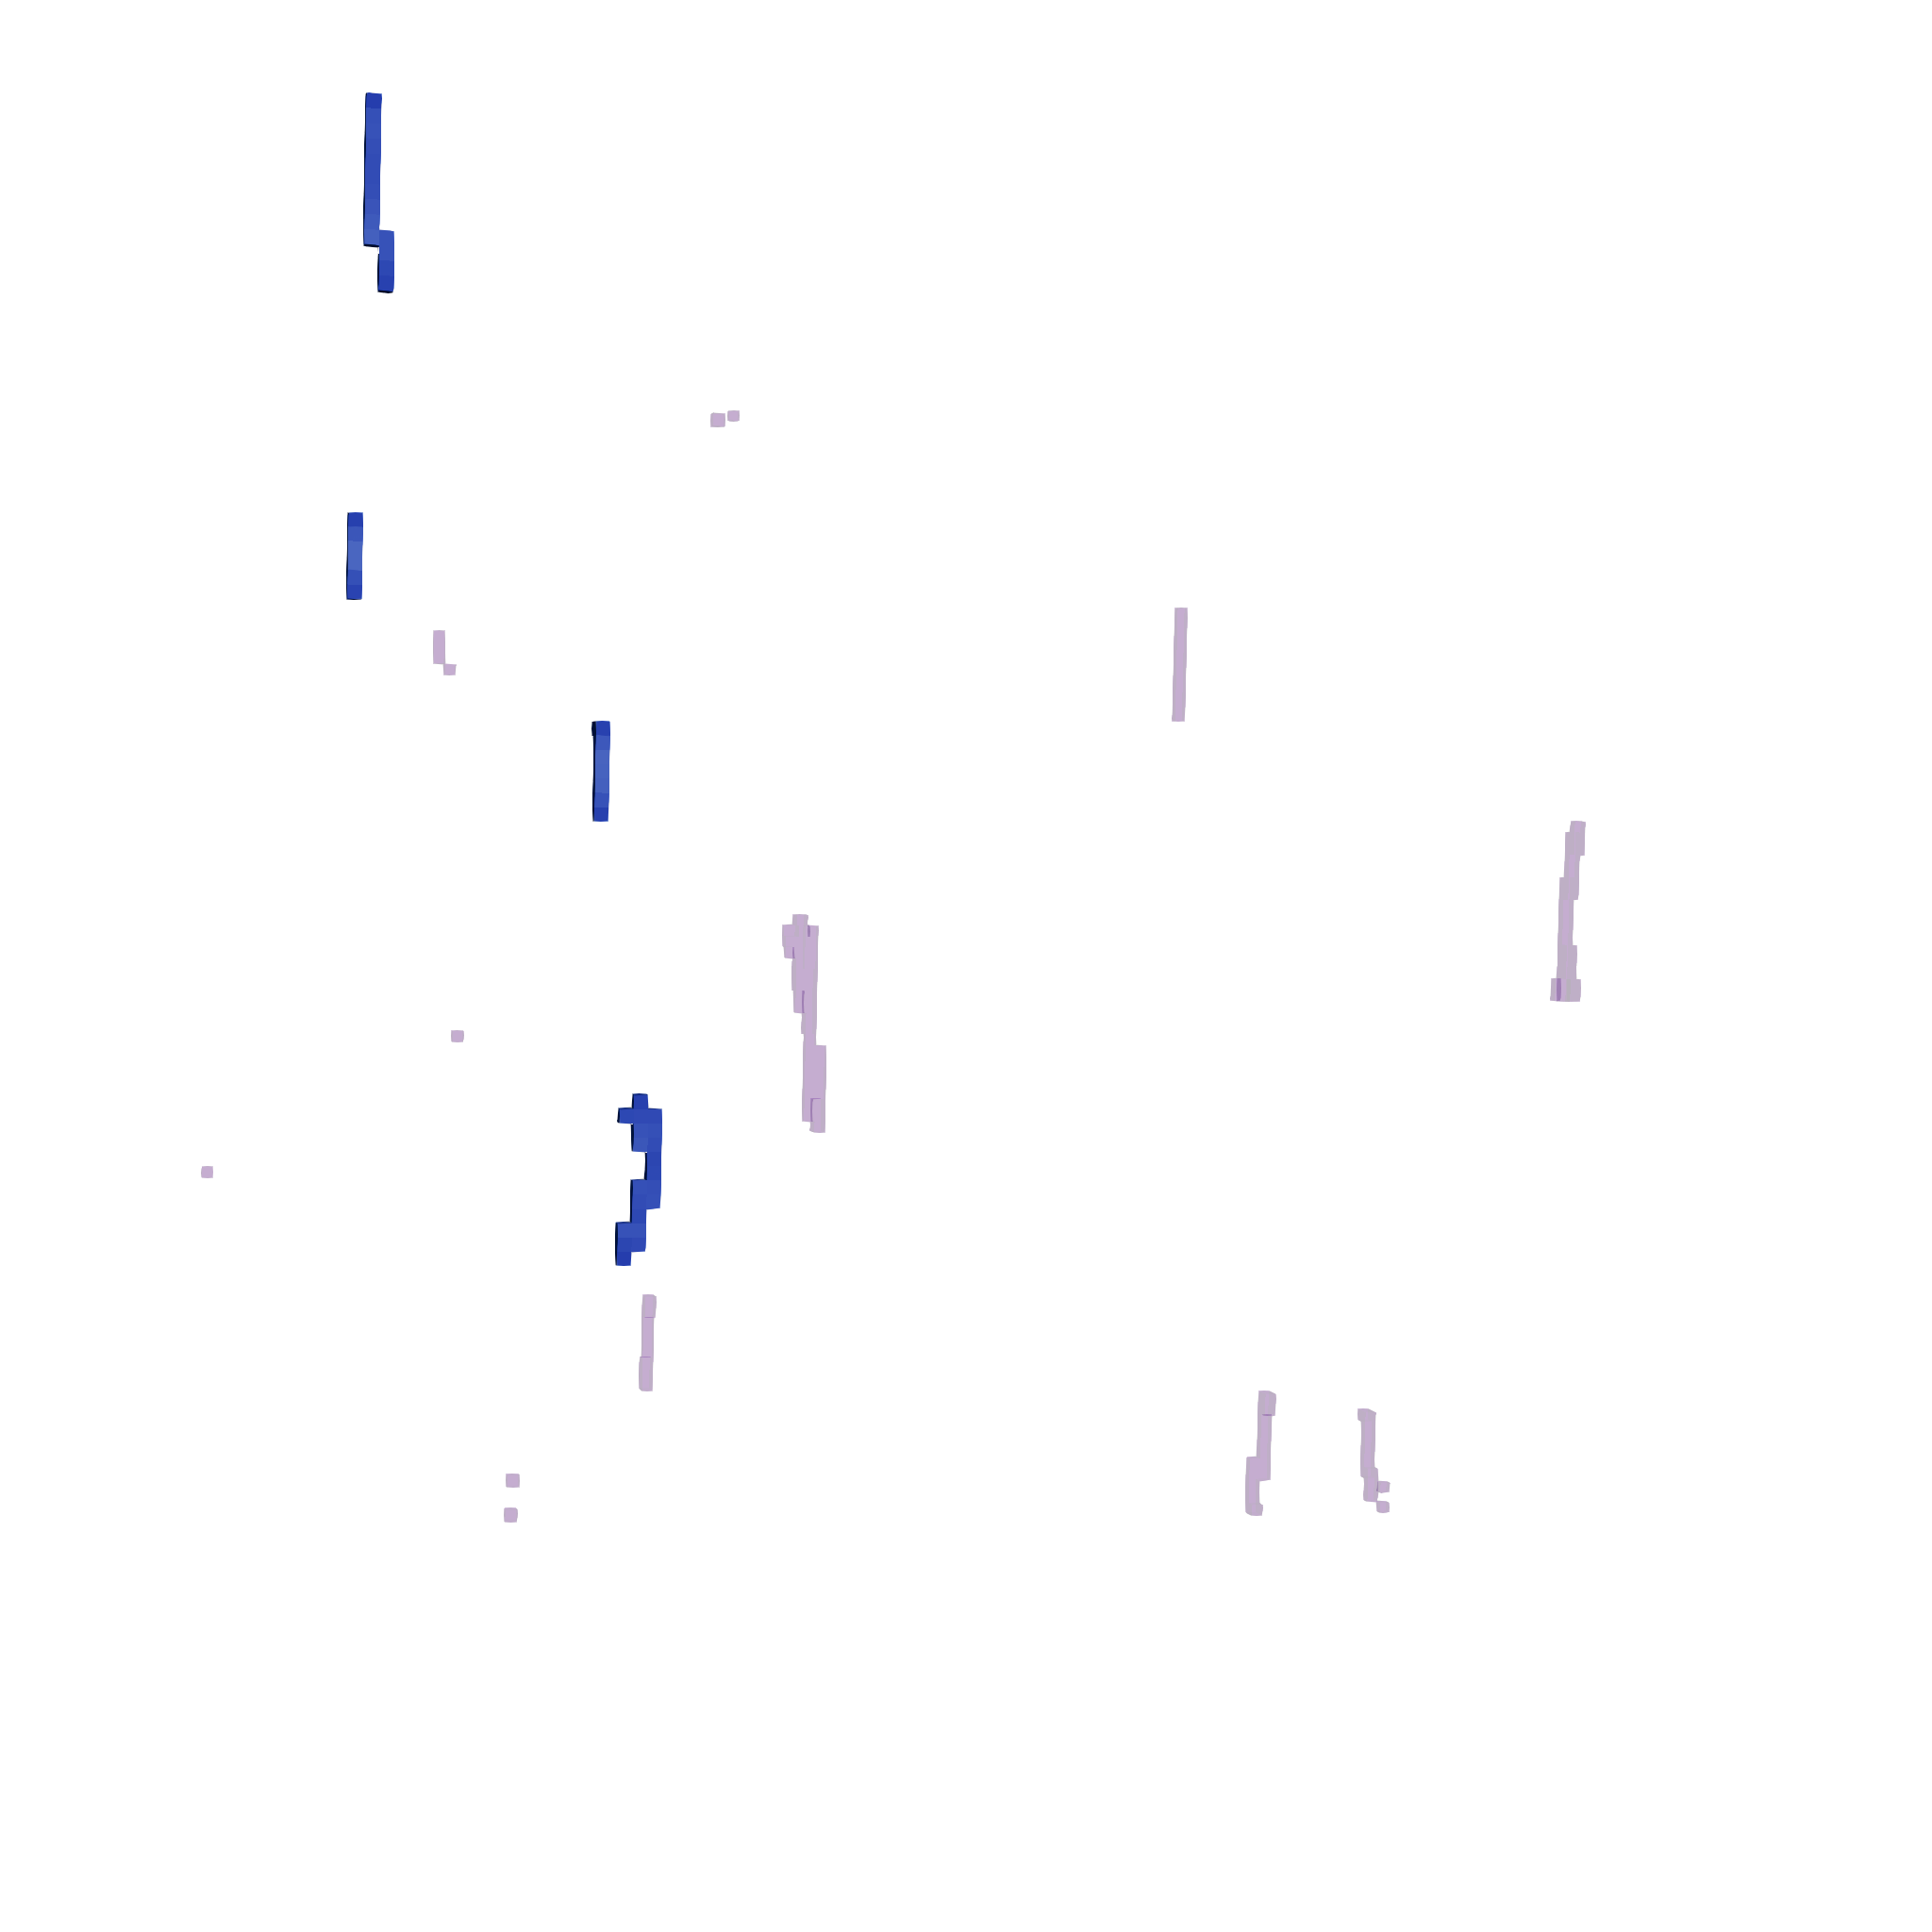
\includegraphics[width=0.333\textwidth]{figures/result_disturbance_1.png}}}
	\subfloat[Рост и слияние]{\frame{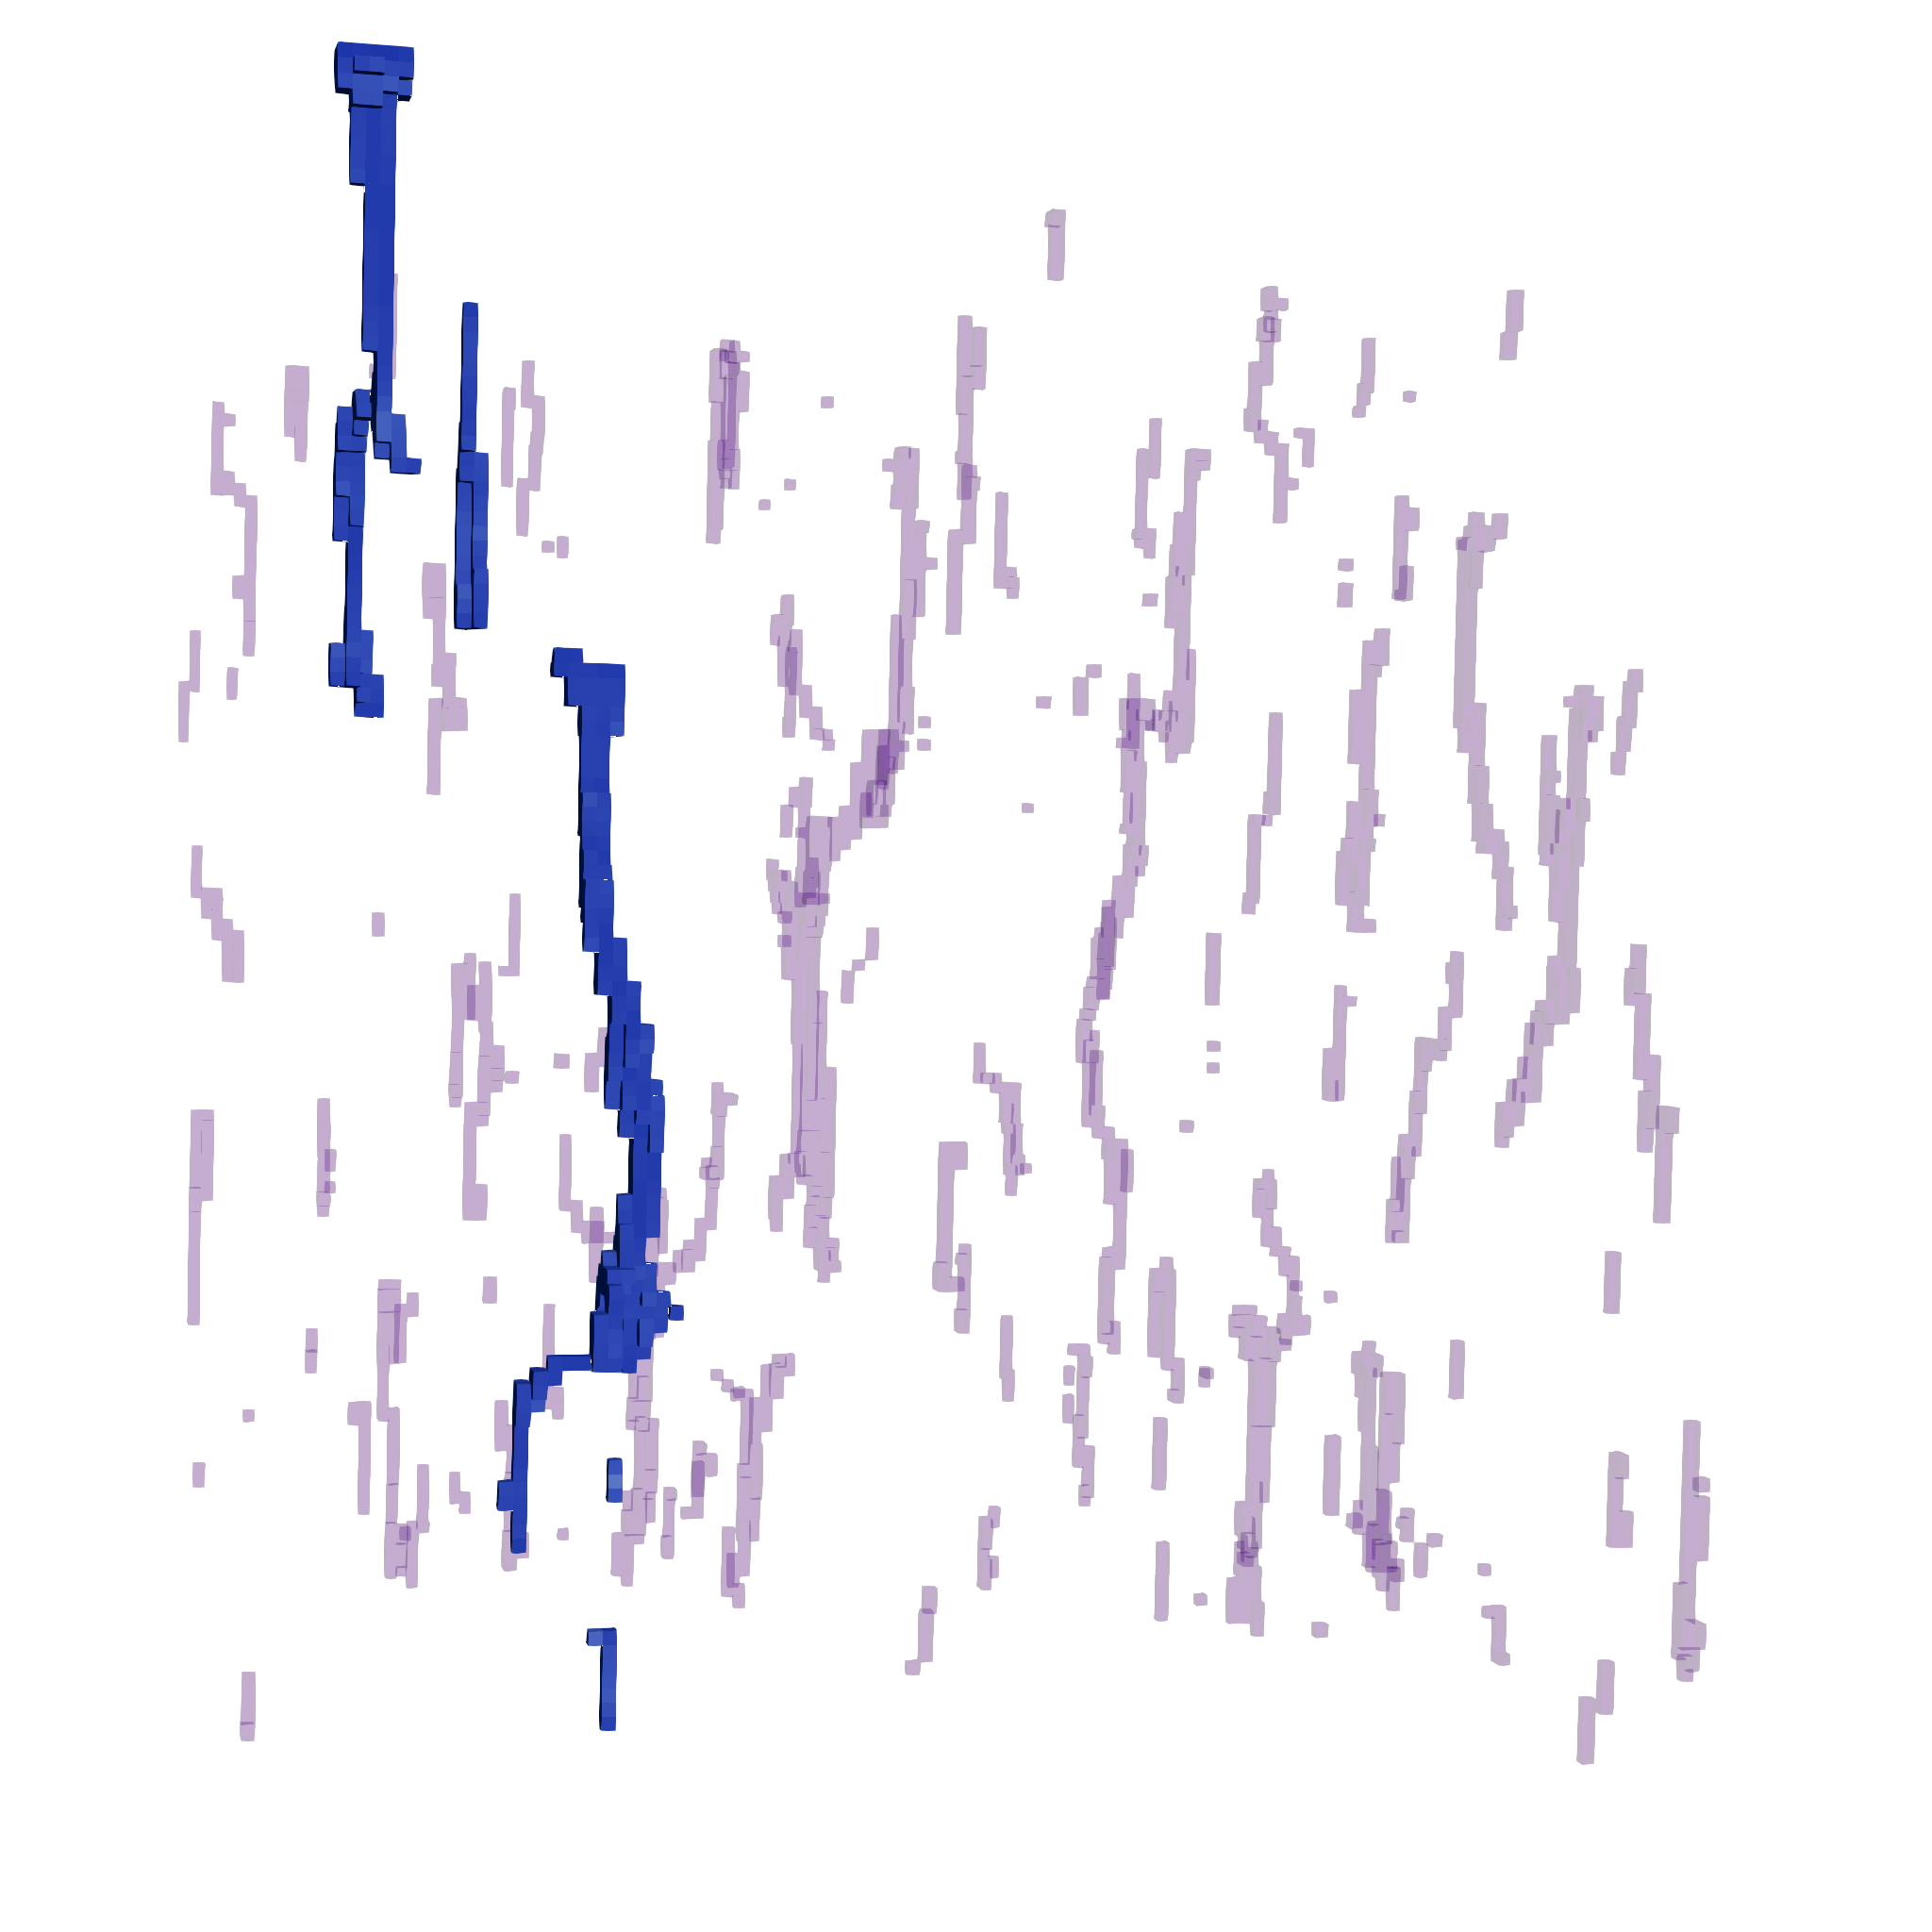
\includegraphics[width=0.333\textwidth]{figures/result_disturbance_2.png}}}
	\subfloat[Пробой <<насквозь>>]{\frame{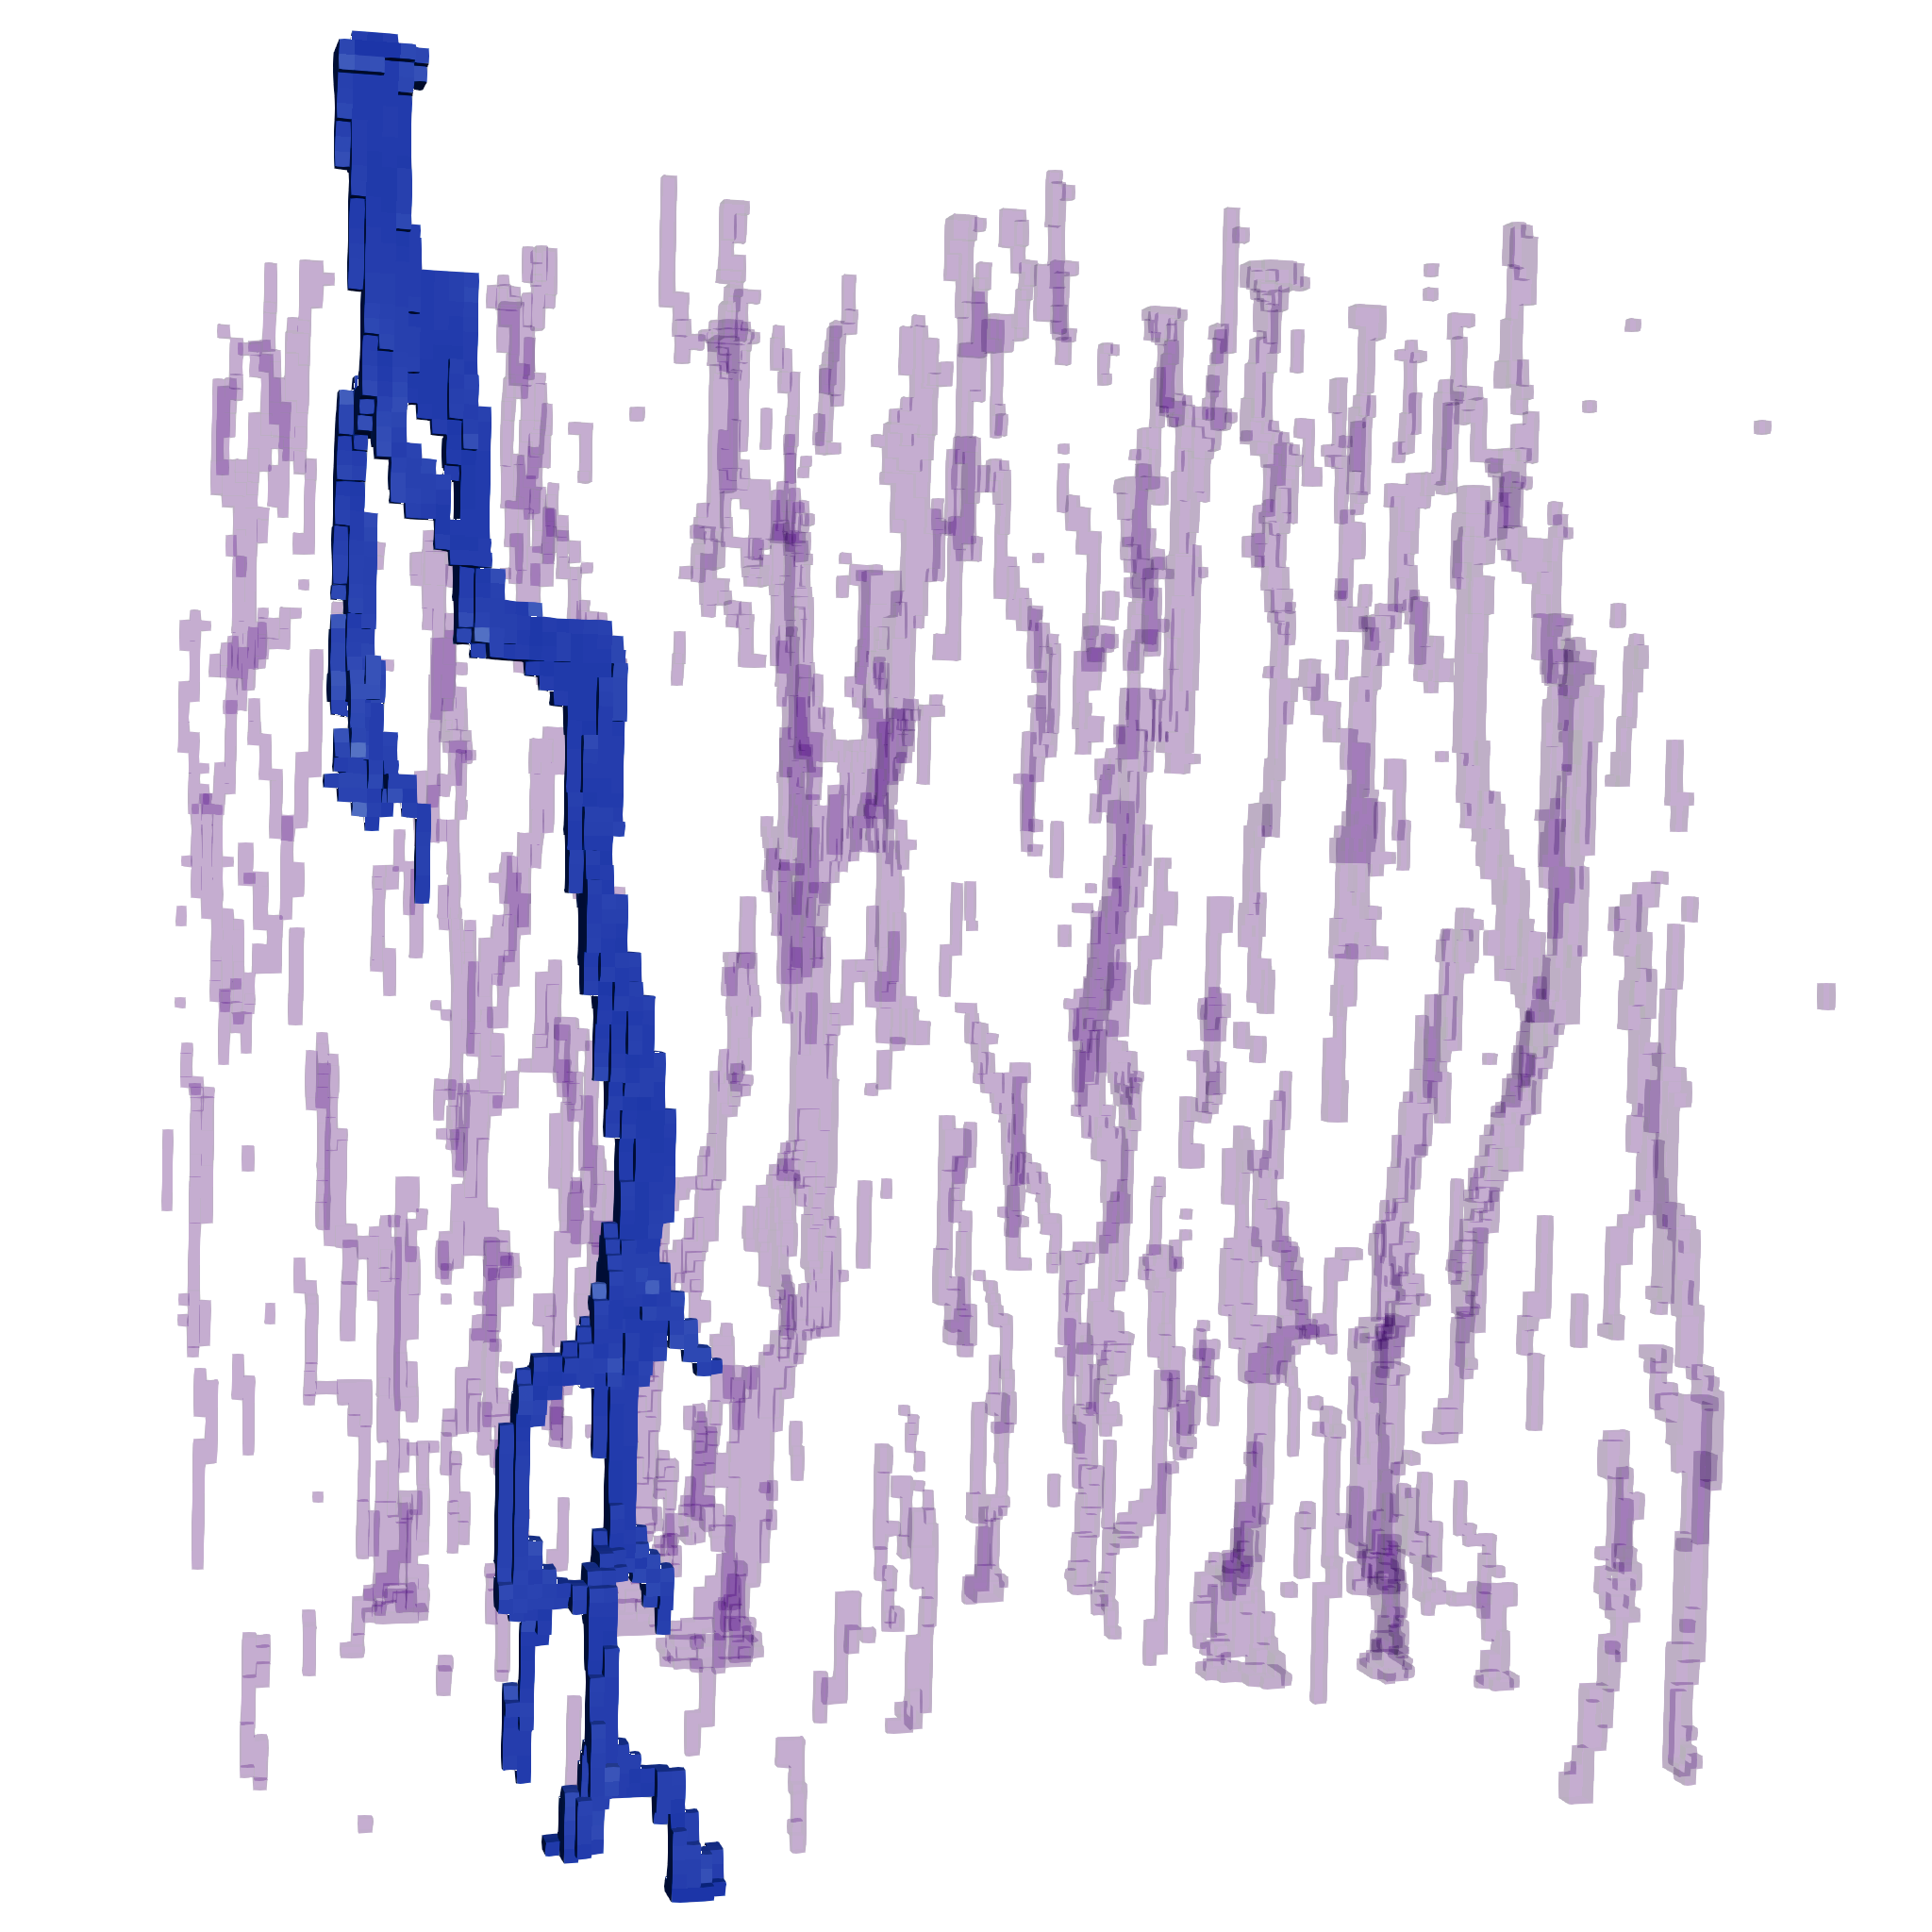
\includegraphics[width=0.333\textwidth]{figures/result_disturbance_3.png}}}
\end{figure}
\vspace{-7mm}
\begin{minipage}[l]{0.66\textwidth}
\begin{align*}
	N_h &= 129 & T &\approx 1.7 \cdot 10^{-6} & \taumin &= 10^{-12} \\
	N_t &= 22000 & \Tol &= 10^{-2} & \taumax &= 10^{-7}
\end{align*}
\end{minipage}
\end{frame}


\begin{frame}{Литература}
\printbibliography
\end{frame}

\begin{frame}{}
\begin{center}
	\Large
	Спасибо за внимание!
\end{center}
\end{frame}

\end{document}